% Copyright 2007 by Till Tantau
%
% This file may be distributed and/or modified
%
% 1. under the LaTeX Project Public License and/or
% 2. under the GNU Public License.
%
% See the file doc/licenses/LICENSE for more details.


\lecture[review]{Sum-up and review}{lecture-body}

\date{5 December 2013}


\begin{document}

\begin{frame}\frametitle<presentation>{Outline}
  \begin{enumerate}
    \item General principles
    \item Test
    \item What you should know for each test
    \item Other concepts
  \end{enumerate}
\end{frame}


%%%%%%
\begin{frame}{General Principles}

  \begin{itemize}
    \item always look at, and think about, the data
    \item correlation is not causation (consider confounding factors)
    \item  sample size is like a magnifying glass, it lets you see smaller effect sizes
    \item  ... but statistical significance does not imply real-world importance
    \item  statistical (hypothesis) tests have two pieces: a test statistic, and a null model
    \item  the P-value is the probability of seeing a test statistic at least as extreme under the null model
    \item  nonindependent observations can drastically mislead you
    \item  if the sampling distribution is not close to Normal, use a distribution-free test
  \end{itemize}


\end{frame}


%%%%%%
\begin{frame}{Tests}

  \begin{itemize}
    \item two-sample t-test
    \item Wilcoxon-Mann-Whitney
    \item paired-sample t
    \item paired-sample sign
    \item Wilcoxon sign-rank
    \item CI for estimated proportion
    \item chi-squared for single-sample proportions
    \item two-sample chi-squared
    \item F-test for one-way ANOVA
    \item F-test for two-way ANOVA
    \item t-test for no linear correlation
  \end{itemize}

\end{frame}

%%%%%%
\begin{frame}{What you should know for each test}

  \begin{itemize}
    \item what sort of data the test applies to
    \item what conditions the test needs to be appropriate
    \item how to check the conditions are satisfied
    \item how to formulate the null \& alternative hypotheses
    \item what the test statistic is and how to compute it
    \item how to interpret the result, statistically, and in real-world terms
  \end{itemize}


\end{frame}

%%%%%%
\begin{frame}{Other concepts}
  
  \begin{itemize}
    \item standard deviation of --
    \item standard error of --
    \item effect size (of difference in means)
    \item back-calculation of necessary sample size to have power to see a certain effect (e.g. for differences in proportion)
    \item the two-way ANOVA model: group means, interaction means, plus noise/variability
    \item correlation: proportion of variance explained
    \item the linear (regression) model: linear conditional men plus noise/variability
    \item regression: residuals, leverage, influence
  \end{itemize}


\end{frame}

\end{document}

%%%%%%
\begin{frame}{Example}

  Lactate dehydrogenase levels:
  \begin{center}
    \begin{tabular}{crr}
       & Males & Females \\
       \hline
       $n$ & 270 & 264 \\
       $\bar y$ & 60 & 57 \\
       $s$ & 11 & 10
     \end{tabular}

   \vspace{2em}

   \uncover<2->{$t_s=3.3$ and $P=0.001$}
   \end{center}

\end{frame}



%%%%%%
\begin{frame}{Example}

  Body weight:
  \begin{center}
    \begin{tabular}{crr}
       & Males & Females \\
       \hline
       $n$ & 2 & 2 \\
       $\bar y$ & 175 & 143 \\
       $s$ & 35 & 34
     \end{tabular}

   \vspace{2em}

   \uncover<2->{$t_s=0.93$ and $P=0.45$}
   \end{center}

\end{frame}


%%%%%%
\begin{frame}{Example: soil respiration}

  Soil cores from two locations, ``gap'' and ``growth'';
  measured amount of CO${}_2$ released.

  \begin{center}
  \begin{tabular}{l|p{2.5in}}
    growth & 17 \hspace{.25em} 20 \hspace{.25em} 170 \hspace{.25em} 315 \hspace{.25em} 22 \hspace{.25em} 190 \hspace{.25em} 64 \\
    \hline
    gap & 22 \hspace{.25em} 29 \hspace{.25em} 13 \hspace{.25em} 16 \hspace{.25em} 15 \hspace{.25em} 18 \hspace{.25em} 14 \hspace{.25em} 6 \\
  \end{tabular}

    \vspace{2em}

    \structure{Exercise:} help compute the $P$-value.

    \vspace{2em}


    \uncover<2->{
    % wilcox.test( c(17,20,22,64,170,190,315), c(6,13,14,15,16,18,22,29) ) #= 0.015
    $K_1 = 49.5$ and $K_2 = 6.5$ \\
    $0.009 \le P \le 0.014$
    }
  \end{center}

\end{frame}

%%%%%%
\begin{frame}{Example}

    \structure{Example:} hunger rating with and without mCPP.
    \begin{center}
      \begin{tabular}{lrrr}
        \hline
        subject & mCPP & placebo & difference \\ 
        \hline
        1 & 79 & 78 & 1 \\ 
        2 & 48 & 54 & -6 \\ 
        3 & 52 & 142 & -90 \\ 
        4 & 15 & 25 & -10 \\ 
        5 & 61 & 101 & -40 \\ 
        6 & 107 & 99 & 8 \\ 
        7 & 77 & 94 & -17 \\ 
        8 & 54 & 107 & -53 \\ 
        9 & 5 & 64 & -59 \\ 
        \hline
         Mean & 55 & 85 & -30 \\ 
         SD & 32 & 34 & 33 \\ 
         \hline
      \end{tabular}
    \end{center}
\end{frame}

%%%%%%
\begin{frame}{Example}
    Density of nerves at two sites in the intestine in 9 horses:
    \begin{center}
\begin{tabular}{rrrr}
  \hline
 animal & site I & site II & difference \\ 
  \hline
  1 &  50.60 & 38.00 & +12.60 \\ 
  2 &  39.20 & 18.60 & +20.60 \\ 
  3 &  35.20 & 23.20 & +12.00 \\ 
  4 &  17.00 & 19.00 & -2.00 \\ 
  5 &  11.20 & 6.60 & +4.60 \\ 
  6 &  14.20 & 16.40 & -2.20 \\ 
  7 &  24.20 & 14.40 & +9.80 \\ 
  8 &  37.40 & 37.60 & -0.20 \\ 
  9 &  35.20 & 24.40 & +10.80 \\ 
   \hline
\end{tabular}
    \end{center}

\end{frame}


%%%%%%
\begin{frame}{Example}

    Out of 169 women with family histories of breast cancer, 27 had mutations in the BRCA1 gene.

    \pause
    \vspace{2em}

    \alert{Wilson's estimator} gives that around
        \[ \wt p = \frac{27 + 2}{169+4} = .168 \]
    of women with family histories of breast cancer have mutations in BRCA1.

    \vspace{2em}

    The \alert{standard error} of this estimate is
    \[ \SE_{\wt P} = \sqrt{\frac{.168(1-.168)}{169+4}} = .028  \]

    \vspace{2em}

    A \alert{95\% confidence interval} for this proportion is $\wt p \pm 1.96 \times .028$:
    \[ 0.113 < p < 0.223 \]

\end{frame}

%%%%%%
\begin{frame}{Example}

    Colorblindness in females:
    \begin{center}
        \begin{tabular}{r|rrr}
            & observed counts & expected counts & difference\\
            \hline 
            nonmutant & 850 & 840.9 & 9.1 \\ 
            carrier &  146 & 152.2 & -5.8 \\ 
            colorblind & 4 & 6.9 & 2.9  \\
        \end{tabular}
    \end{center}

    \pause
    \vspace{2em}

    \[
        \chi^2_s = \frac{9.1^2}{840.9} + \frac{5.8^2}{152.2} + \frac{2.9^2}{6.9} .
    \]

\end{frame}

%%%%%%
\begin{frame}{Another example}

    By area, 
    40\% is pavement,
    30\% of a Santa Monica parking lot is shiny cars,
    20\% is dull cars,
    and 10\% is other.\\
    \structure{Hypothesis:} birds don't notice what they are pooping on.
    We counted the numbers of bird poops on each in a given day:
    \begin{center}
        \begin{tabular}{rr}
            & observed counts \\
            \hline 
            pavement & 65 \\
            shiny & 77 \\
            dull & 35 \\
            other & 18 \\
            \hline
            total & 195
        \end{tabular}
    \end{center}

\end{frame}


\begin{frame}{Example}


    \begin{center}
        \begin{tabular}{lcc|c}
            & female & male & total \\
            \hline
            HIV test & 9 & 8 & 17 \\
            no HIV test & 52 & 51 & 103 \\
            \hline
            total & 61 & 59 & 120 \\
        \end{tabular}
    \end{center}

    \vspace{1em}

    \structure{Example:}
    \begin{align*}
        \hat \prob\{ \text{HIV test} \} = \frac{17}{120} \\
        \hat \prob\{ \text{HIV test} \vert \text{female} \} = \frac{9}{61} \\
        \hat \prob\{ \text{HIV test} \vert \text{male} \} = \frac{8}{59} \\
    \end{align*}

\end{frame}

%%%%%%
\begin{frame}{The test statistic}

    Observed (expected) counts:
        \begin{center}
            \begin{tabular}{lcc|c}
                & female & male & total \\
                \hline
                HIV test & 9 (8.64) & 8 (8.36) & 17 \\
                no HIV test & 52 (52.36) & 51 (50.64) & 103 \\
                \hline
                total & 61 & 59 & 120 \\
            \end{tabular}
        \end{center}

    \vspace{2em}

    The test statistic is the \alert{same} as $\chi^2_s$:
    \[
        \chi^2_s = \frac{(9 - 8.64)^2}{8.64} + 
            \frac{(8 - 8.36)^2}{8.36} + 
            \frac{(52 - 52.36)^2}{52.36} + 
            \frac{(51 - 50.64)^2}{50.64} = 0.035
    \]
    and there is \alert{one} {degree of freedom}, and $P > 0.2$ \\
    so there is no significant evidence that men and women get tested at different rates.


\end{frame}

%%%%%%
\begin{frame}{Example: Hair and Eye Color}

    In 6,800 German men, hair (columns) and eye (rows) color were:
        \begin{center}
            \begin{tabular}{l|cccc}
                & brown & black & fair & red \\
                \hline
                brown & 438 & 288 & 115 & 16 \\
                grey/green & 1387 & 746 & 946 & 53 \\
                blue & 807 & 189 & 1768 & 47 \\
            \end{tabular}
        \end{center}

\end{frame}

%%%%%%
\begin{frame}{Example I}

\begin{tabular}{ll|rr}
  value & group & $\bar y_i$ & $y_{ij}-\bar y_i$  \\ 
  \hline
3   &  A  &  5.75  &  -2.75      \\
7   &  A  &  5.75  &  1.25       \\
8   &  A  &  5.75  &  2.25       \\
5   &  A  &  5.75  &  -0.75      \\
6   &  B  &  5.00     &  1.00          \\
5   &  B  &  5.00     &  0.00          \\
5   &  B  &  5.00     &  0.00          \\
10  &  B  &  5.00     &  5.00          \\
2   &  B  &  5.00     &  -3.00         \\
3   &  B  &  5.00     &  -2.00         \\
2   &  B  &  5.00     &  -3.00         \\
7   &  B  &  5.00     &  2.00        \\
   \hline
   & SS & 1.5 & 66.75 \\ 
   & df & 1 & 10 \\ 
   & MS & 0.15 & 6.675   \\ 
\end{tabular}

\end{frame}

%%%%%%
\begin{frame}{Summarized, ANOVA-style}

  \begin{center}
    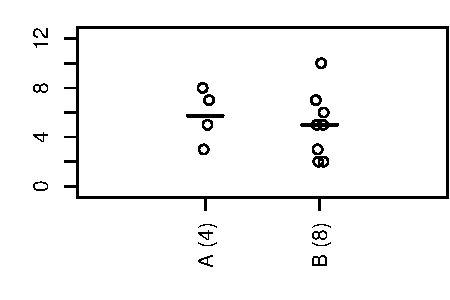
\includegraphics{dots3ex.pdf}

    \vspace{2em}

    \begin{tabular}{lrrr}
      source & df & SS & MS \\
      \hline
      between groups & 1 & 1.5 & 1.5 \\
      within groups & 10 & 66.75 & 6.675 \\
      \hline
      Total & 11 & 68.25 & \\
    \end{tabular}

  \end{center}

\end{frame}

%%%%%%
\begin{frame}{Example of $F$ test}

    Weight gain of lambs on three diets
    \begin{center}
        \begin{tabular}{cccc}
            & diet 1 & diet 2 & diet 3 \\
            \hline
            $n_i$ & 3 & 5 & 4 \\
            $\bar y_i$ & 11 & 15 & 12 \\
            $s_i$ & 4.359 & 4.950 & 4.967 \\
        \end{tabular}
    \end{center}

    \pause

    \begin{center}
        \begin{tabular}{cccc}
            & df & $\SS$ & $\MS$ \\
            between diets & 2 & 36 & 18 \\
            within diets & 9 & 210 & 23.33 \\
            \hline
            total & 11 & 246 & \\
        \end{tabular}
    \end{center}


    \vspace{2em}

    With $df = (2,9)$ and
    \[ F_s = \frac{ 18 }{ 23.33 } = 0.77 , \]
    we find that $P > 0.20$.


    \vspace{2em}

    \pause
    There is not good evidence that diet affects the weight gain of lambs.


\end{frame}

%%%%%%
\begin{frame}{Example: beak size}

    Beak size of finches in different islands:

    { \tiny
\begin{tabular}{c|cccccccccc}
    &   a & a & b & b & c & c & d & d & e & e \\
    &   F & M & F & M & F & M & F & M & F & M \\
    \hline
    & 10.10  &  10.66  & 11.86  &  14.67  &  10.07  & 12.95  &  11.51  &  14.60  &   12.74  & 14.33  \\
    & 9.32   &  13.31  & 14.14  &  14.60  &  10.34  & 11.39  &  13.15  &  13.88  &   13.83  & 16.18  \\
    & 8.42   &  11.88  & 10.72  &  13.97  &  8.42   & 10.86  &  12.93  &  12.48  &   12.91  & 16.42  \\
    & 7.72   &  9.88   & 13.11  &  12.55  &  8.93   & 11.09  &  13.44  &  13.58  &   13.12  & \\
    & 10.04  &  10.85  & 10.14  &  12.60  &  10.20  & 10.95  &  12.91  &  12.76  &          & \\
    & 10.24  &  11.70  & 11.20  &         &   10.93  & 9.39   &  13.08  &  14.51  &          & \\
    & 10.32  &  10.94  & 13.68  &         &   10.29  &        &   12.49  &  14.55  &          & \\
    &        &   9.72   & 12.30  &         &   11.34  &        &   13.19  &  14.81  &          & \\
    &        &   11.03  & 11.12  &         &          &         &   12.54  &  13.20  &          & \\
    &        &   10.87  & 13.24  &         &          &         &   11.29  &  13.83  &          & \\
    &        &   9.55   & 11.99  &         &          &         &   13.45  &  15.05  &          & \\
    &        &          &  10.57  &         &          &         &   11.61  &         &           & \\
    &        &          &         &          &          &         &   14.43  &         &           & \\
   \hline
$n_i$  &  7     &  11     &  12     &  5      &  8      &  6      &  13     &  11     &  4      &  3      \\
mean   &  9.45  &  10.94  &  12.00  &  13.67  &  10.06  &  11.10  &  12.76  &  13.93  &  13.14  &  15.64  \\
SD     &  1.01  &  1.08   &  1.30   &  1.04   &  0.96   &  1.14   &  0.88   &  0.85   &  0.48   &  1.14   \\
\end{tabular}
}
\end{frame}

%%%%%%
\begin{frame}{$F$-tests, summary:}

  \begin{center}
    \begin{tabular}{c|ccccc}
 & df & Sum Sq & Mean Sq & F value & $P$  \\
 \hline
island & 4 & 173.912 & 43.478 & 41.0228 & $<$.000001 \\
sex & 1 & 23.032 & 23.032 & 21.7317 & .000014 \\
interaction & 4 & 3.102 & 0.776 & 0.7318 & 0.5733  \\
within & 70 & 74.189 & 1.060 &  & \\
\hline
total & 79 & 274.235 & & & \\
\end{tabular}
\end{center}


    \vspace{2em}

    \structure{Conclusion:} We have very strong evidence that mean beak size varies between sexes, and by island, but have no evidence that these effects are not additive.

\end{frame}

%%%%%%
\begin{frame}{Example:}

  \textit{Toxoplasma gondii} infection rates and measures of aggregate neuroticism in 31 countries:

  \begin{center}
    \only<1>{
    \scriptsize
\begin{tabular}{lrr|lrr}
  \hline
  country & prevalence (\%) & N18 &
  country & prevalence (\%) & N18 \\ 
  \hline
Argentina    &  52.70  &  51.30   & Japan        &  12.30  &  50.70  \\
Australia    &  28.00  &  48.60   & Netherlands  &  24.50  &  48.60  \\
Austria      &  36.00  &  48.30   & Norway       &  8.60   &  47.40  \\
Belgium      &  46.80  &  49.60   & Peru         &  32.90  &  48.50  \\
Brazil       &  66.90  &  53.70   & Poland       &  46.50  &  50.70  \\
China        &  24.30  &  53.10   & SouthKorea   &  4.30   &  48.40  \\
Croatia      &  37.40  &  49.30   & Slovenia     &  30.90  &  50.60  \\
CzechRep     &  26.60  &  51.40   & Spain        &  22.70  &  49.70  \\
Denmark      &  22.00  &  50.30   & Sweden       &  12.50  &  46.30  \\
Ethiopia     &  16.40  &  48.80   & Switzerland  &  36.70  &  47.50  \\
France       &  45.00  &  52.70   & Thailand     &  11.20  &  48.90  \\
Germany      &  42.70  &  48.10   & Turkey       &  46.80  &  51.40  \\
Hungary      &  58.90  &  53.80   & UK           &  6.60   &  50.10  \\
Indonesia    &  46.20  &  50.00   & USA          &  12.30  &  48.10  \\
Ireland      &  25.00  &  50.10   & Yugoslavia   &  66.80  &  51.10  \\
Italy        &  32.60  &  52.60   &  & & \\
   \hline
\end{tabular}
\figcaption{Lafferty 2006, ``Can the common brain parasite, \textit{Toxoplasma gondii}, influence human culture? ''}
    }
    \only<2>{
    \includegraphicscopyright{ex24-toxo}{Lafferty 2006, ``Can the common brain parasite, \textit{Toxoplasma gondii}, influence human culture? ''}
    }
    \only<3>{
    \includegraphicscopyright{ex24-toxo-line}{Lafferty 2006, ``Can the common brain parasite, \textit{Toxoplasma gondii}, influence human culture? ''}
    }
  \end{center}

\end{frame}



